\newpage
\maketitle
\begin{center}
\Large \textbf{第1章 强化学习概述} \quad 
\end{center}
\begin{abstract}
在本章中我们将讨论强化学习中的环境、Agent、状态、Action和奖励,并重点讨论MDP相关内容。
\end{abstract}
\section{MDP概述}
一个典型的强化学习系统结构如下所示:
\begin{figure}[H]
	\caption{典型强化学习系统架构图}
	\label{p000001}
	\centering
	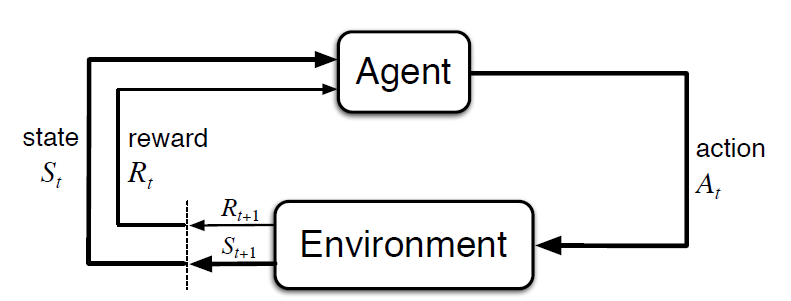
\includegraphics[width=15cm]{images/p000001}
\end{figure}
如图所示:
\begin{enumerate}
    \item 在$t$时刻Agent观察到环境状态$S_{t}$,并得到上一时刻所采取的行动$A_{t-1}$(在图中未画出)所得到的
奖励$r_{t}$;
    \item Agent根据环境状态$S_{t}$,根据某种策略$\pi$,选择行动$A_{t}$;
    \item 环境接收到Agent的行动$A_{t}$后,根据环境的动态特性,转移到新的状态$S_{t+1}$,并产生$R_{t}$的奖励
信号;
\end{enumerate}
\subsection{典型环境}
\subsubsection{Bandit Walk环境}
下面我们来研究一个最简单的强化学习环境,叫Bandit Walk,如下所示:
\begin{figure}[H]
	\caption{Bandit Walk环境图}
	\label{p000002}
	\centering
	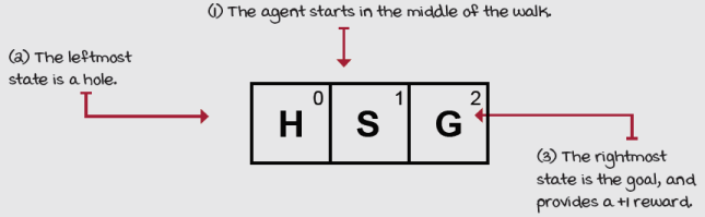
\includegraphics[width=15cm]{images/p000002}
\end{figure}
如图所示,Agent初始时位于中间的S格,状态编号为$S_{0}$,其可以采取向左、向右两个动作,向左则进入状态$H$,其是一个洞,就会掉到洞里,
过程就会结束,此时得到的奖励为0;当Agent采取向右行动时,就会进入G状态,此时会获得奖励+1,由此可见其是一个确定性的环境,就是说当
Agent采取向右行动时,会100\%确定进行G状态。我们可以通过如下的图来表示上述过程:
\begin{figure}[H]
	\caption{Bandit Walk环境MDP图}
	\label{p000003}
	\centering
	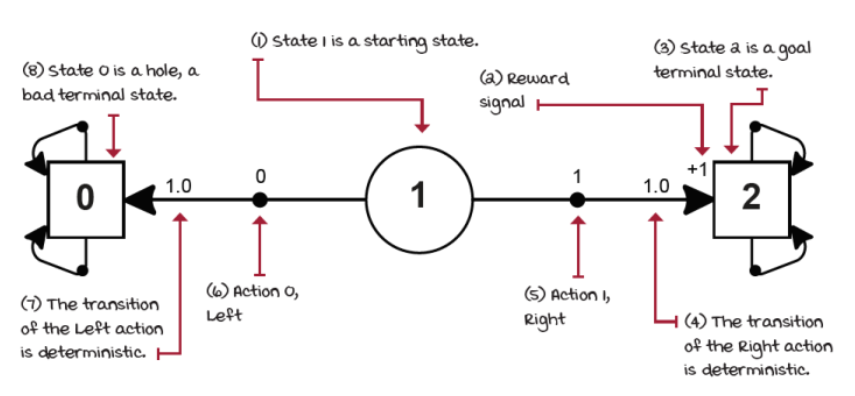
\includegraphics[width=15cm]{images/p000003}
\end{figure}
如图所示:
\begin{itemize}
    \item 在初始状态$S_{0}$时,有两个可选行动,分别表示为向左、向右的直线;
    \item 当采取向右行动时,就会到达小黑点位置,然后由环境决定将转到哪个状态,以及转到这个状态的概率,以本例为例,其就是以100\%
的概率转到G状态$S_{2}$,其中小黑点上面的1代表行动编号,向右简头上面的1.0代表100\%的概率,向右简头处的1代表奖励为+1;
\end{itemize}
我们首先安装所需要的库:
\lstset{language=PYTHON, caption={安装gmy库}, label={pip-install-gym}}
\begin{lstlisting}
pip install -i https://pypi.tuna.tsinghua.edu.cn/simple gym
\end{lstlisting}
下面我们用Python对象来表示这一过程:
\lstset{language=PYTHON, caption={Bandit Walk python程序}, label={bandit-walk-python-env}}
\begin{lstlisting}
P = {
    0: {
        0: [(1.0, 0, 0.0, True)],
        1: [(1.0, 0, 0.0, True)]
    },
    1: {
        0: [(1.0, 0, 0.0, True)],
        1: [(1.0, 2, 1.0, True)]
    },
    2: {
        0: [(1.0, 2, 0.0, True)],
        1: [(1.0, 2, 0.0, True)]
    }
}
print(P)
\end{lstlisting}
代码解读如下所示:
\begin{itemize}
    \item P为一个字典对象,其键值0、1、2代表三个状态;
    \item P的键值0:其同样是一个字典对象,键值代表可以采取的行动,0代表向右,1代表向右;
    \item P的键值0下键值0:即在状态0下面采取行动0,其值为一个数组,代表由环境决定要转到哪个状态,转到每个状态为一个Turple,含
义为:(概率, 目的状态,获得奖励,新状态是否为终止状态),注意:我们规定在终止状态采取任何行动都会回到自身;
\end{itemize}
上面我们仅举了一个例子,其他状态读者可以自己解析出来。
\subsubsection{Bandit Slippery Walk环境}
在上面的环境中,我们向左移动,环境会确定地向左移动。但是在本节中,当我们向左移动时,环境在80\%的情况下会向左移动,20\%的情况会
向右移动。如下图所示:
\begin{figure}[H]
	\caption{Bandit Slippery Walk环境图}
	\label{p000004}
	\centering
	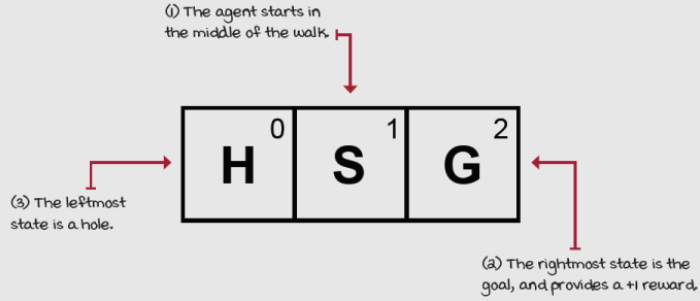
\includegraphics[width=15cm]{images/p000004}
\end{figure}
除了环境的随机性之外,环境与上一节相同。其MDP图如下所示:
\begin{figure}[H]
	\caption{Bandit Slippery Walk环境MDP图}
	\label{p000005}
	\centering
	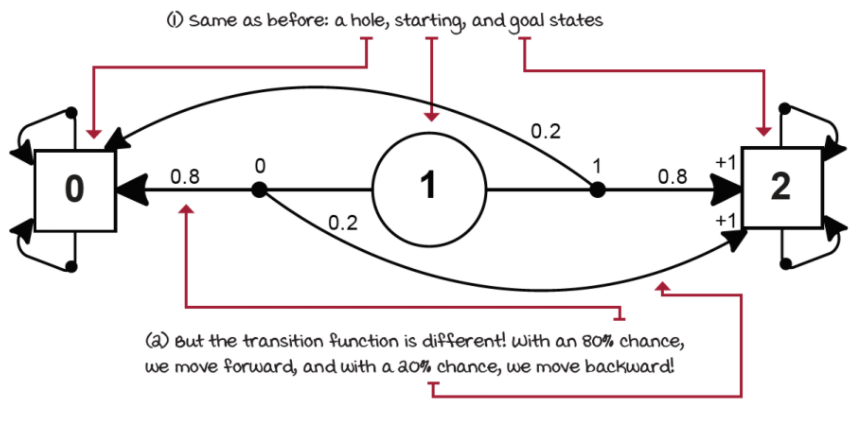
\includegraphics[width=15cm]{images/p000005}
\end{figure}
如上图所示,在开始时Agent位于状态S,其可以采取的行动为向左编号为0或向右编号为1,我们以向右为例,当Agent采取向右行动时,其达到状态S右侧的小黑点,上面的1代表是编号为1的行动,
此时环境将以80\%的概率转变为状态G,得到+1的奖励,如图中的右箭头所示,同时环境还可能将以20\%的概率变为状态H,其所获得的奖励为0,如图中向左的曲线箭头所示。读者可以按照上面
的描述,自己补充出其他状态变化情况。由前面的讨论可以看出,在这个例子中,当Agent采取向右行动Action时,环境仅以80\%的概率完成该Action,同时还可能以20\%的概率向相反的方向
变化,既环境具有一定的随机性。
我们可以通过如下的Python代码来表示这一过程:
\lstset{language=PYTHON, caption={Bandit Slippery Walk python程序}, label={bandit-slippery-walk-python-env}}
\begin{lstlisting}
    def bandit_slippery_walk(self):
        P = {
            0: {
                0: [(1.0, 0, 0.0, True)],
                1: [(1.0, 0, 0.0, True)]
            },
            1: {
                0: [(0.8, 0, 0.0, True), (0.2, 2, 1.0, True)],
                1: [(0.8, 2, 1.0, True), (0.2, 0, 0.0, True)]
            },
            2: {
                0: [(1.0, 2, 0.0, True)],
                1: [(1.0, 2, 0.0, True)]
            }
        }
        print(P)
\end{lstlisting}
如上所示,在状态S时,如果采取编号为0的向左行动,则有80\%的概率会进入到状态H,奖励为0.0,并且是终止状态,当采用编号为1的向右行动时,将进入状态G,获得奖励为1.0,并且为终止状态,
采用这种方式我们就表示了环境的随机性。
\subsection{典型交互}
Agent与环境的交互分为分段的或连续的,由一系列时间步聚组成,在时间$t$时刻:
\begin{itemize}
    \item Agent得到环境给的奖励信号$R_{t}$,其由Agent在上一时刻$S_{t-1}$采取行动$A_{t-1}$时所获得的,并且Agent观察到环境状态$S_{t}$;
    \item Agent根据所观察到的环境状态$S_{t}$,选择采取行动$A_{t}$;
    \item 环境接收到行动$A_{t}$后,会转移到新的状态$S_{t+1}$,并且会给Agent奖励$R_{t+1}$;
    \item 依次循环......
\end{itemize}
上述过程可以表示为:
\begin{equation}
\begin{aligned}
(R_{0}, S_{0}, A_{0}), (R_{1}, S_{1}, A_{1}), (R_{2}, S_{2}, A_{2}), ..., (R_{t}, S_{t}, A_{t}), ..., (R_{T}, S_{T}, A_{T})
\end{aligned}
\label{mdp-episode-trajectory}
\end{equation}
\subsection{MDP定义}
我们以Frozen Lake为例来定义MDP过程。该环境如下所示:
\begin{figure}[H]
	\caption{Frozen Lake环境图}
	\label{p000006}
	\centering
	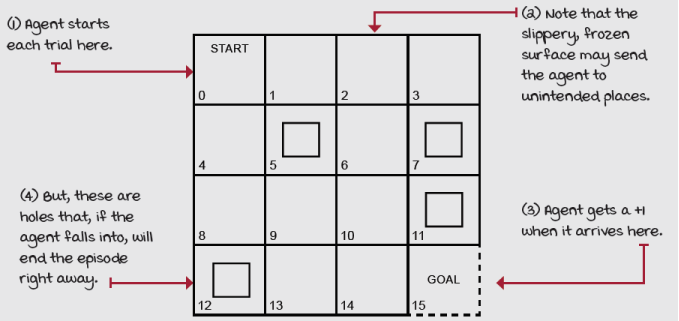
\includegraphics[width=15cm]{images/p000006}
\end{figure}
如图所示:
\begin{itemize}
    \item Agent从状态Start开始;
    \item 在每个状态,Agent可以采取向左、向上、向下、向右行动,当在边缘状态时,走出环境的行动会100\%使Agent留在原状态;
    \item 由于是冻冰的湖面,例如当Agent选择向下行动时,其有33.3\%的概率向下运动,还有66.7\%的概率会向垂直的方向运动,既以33.3\%的概率向左运动,33.3\%的概率向右运动;
    \item 当Agent到达有洞的状态时,过程立即结束;
    \item 当Agent到达最终节点时,可以获得+1的奖励;
\end{itemize}
\subsubsection{环境状态建模}
时刻$t$环境状态的状态表示为$S_{t}$,环境所有可能的状态用集合$\mathcal{S}$表示,通常我们用$n$维向量来表示一个状态:
\begin{equation}
\begin{aligned}
S_{t}=\boldsymbol{s} = \begin{bmatrix}
    s_{1} \\
    s_{2} \\
    ... \\
    s_{n}
\end{bmatrix} \in R^{n}
\end{aligned}
\label{state-vector-representation}
\end{equation}
对于我们当前研究的这个问题,环境状态只需要表示Agent处于哪个状态即可,我们采用0$\sim$15来对状态进行编号,因此状态可以用0$\sim$15来表示:
\begin{equation}
\begin{aligned}
S_{t}=\boldsymbol{s} = \begin{bmatrix}
    i
\end{bmatrix} \in R^{1}, i \in \{0, 1, 2, 3, ..., 15\}
\end{aligned}
\label{frozen-lake-state-demo}
\end{equation}
我们规定环境只与当前状态有关,而与过去的历史无关,这就是马可夫特性,即我们研究的过程是无记忆的。乍一看,这是一个非常严重的限制条件,但是在实际应用中,我们通常可以通过设计合适的状态,使
所研究的问题变为无记忆的。用数学语言可以表示为:
\begin{equation}
\begin{aligned}
P(S_{t+1} | S_{t}, A_{t}) = P(S_{t+1} | S_{t}, A_{t}, S_{t-1}, A_{t-1}, ...)
\end{aligned}
\label{markov-property-def}
\end{equation}
以Frozen Lake为例,其每个状态和在状态上可以采取的行动如下所示:
\begin{figure}[H]
	\caption{Frozen Lake状态和行动图}
	\label{p000007}
	\centering
	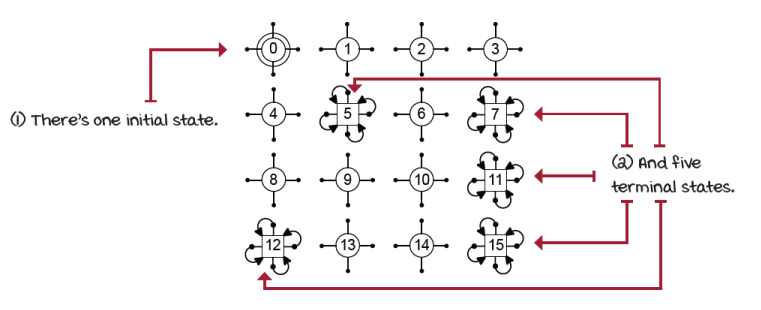
\includegraphics[width=15cm]{images/p000007}
\end{figure}
当Ageng采取行动后,环境会根据自身的动态特性,转移到下一个状态,我们称之为转移函数,如下图所示:
\begin{figure}[H]
	\caption{Frozen Lake状态转移图}
	\label{p000008}
	\centering
	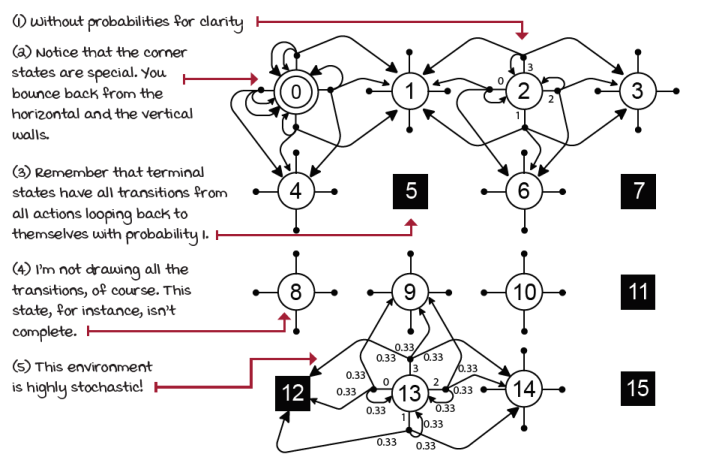
\includegraphics[width=15cm]{images/p000008}
\end{figure}
在状态13时,共有向左、向下、向右、向上编号分别为0、1、2、3的四种行动,当Agent采取行动0向左时,将到达左侧的小黑点,
\begin{itemize}
    \item 行动0(向左):到达左侧小黑点,由于冻冰原因,其有如下三种可能性:
    \begin{itemize}
        \item 33.3\%:向左,进入状态12,获取奖励0.0,并且为终止状态,用(0.333, 12, 0.0, True)表示;
        \item 33.3\%:向下,由于是边缘节点,其仍然在状态13,获取奖励0.0,不为终止状态,用(0.333, 13, 0.0, False)表示;
        \item 33.3\%:向上,进入状态9,获取奖励为0.0,不是终止状态,用(0.33, 9, 0.0, False)表示;
    \end{itemize}
    \item 行动1(向下):到达下面小黑点,有如下三种可能性:
    \begin{itemize}
        \item 33.3\%(向下):由于是边缘节点,其仍然在状态13,获得奖励为0.0,不是终止状态,用(0.333, 13, 0.0, False)表示;
        \item 33.3\%(向左):进入状态12,获得奖励0.0,并且为终止状态,用(0.333, 12, 0.0, True)表示;
        \item 33.3\%(向右):进入状态14,获得奖励0.0,不是终止状态,用(0.333, 14, 0.0, False)表示;
    \end{itemize}
\end{itemize}
我们这里仅举了两个例子,其余内容读者可以自己补全。
环境的状态转移函数如下所示:
\begin{equation}
\begin{aligned}
p(s' | s, a) = P(S_{t}=s' | S_{t-1}=s, A_{t-1}=a) \\
\sum_{s' \in S} p(s' | s, a) = 1, \forall s \in S, \forall a \in A(s)
\end{aligned}
\label{env-state-transition-function}
\end{equation}
上式表明在任意时刻,环境状态为$S_{t-1}=s$,Agnet采取行动为$A_{t-1}=a$时,环境由于具有随机性,以一个确定的概率分布进入新状态$S_{t}=s'$,并且
如果我们将所有可能到达的新状态的概率相加,其值为1。
当Agent根据自己的策略,在任意时刻采取行动后,系统会给Agent一个奖励Reward,其是一个标量,越大代表该行动决策越好,越小代表越差,甚至可以为负值,代表需要尽力避免
的情况。需要注意的是,Agent不仅要关注当前获得的奖励,还要关注最终获得的累积的奖励,Agent的目标就是使最终获得的累积奖励最大。
环境的奖励函数如下表示:
\begin{equation}
\begin{aligned}
r(s, a) = E\bigg( R_{t} | S_{t-1}=s, A_{t-1}=a \bigg)
\end{aligned}
\label{env-reward-function}
\end{equation}
上式表明在$t-1$时刻,环境状态为$S_{t-1}=s$,Agent采取行动$A_{t-1}=a$,环境在$t$时刻给出奖励$R_{t}$,由于环境具有随机性,环境可能进入不同的状态,从而获得不同的奖励,
而且即使是进入同一个状态,获得的奖励也有可能不同,因此在这种情况,下的奖励就是所有这种情况下获得奖励的期望值。
在$t-1$时刻,环境状态为$S_{t-1}=s$,Agent采取行动$A_{t-1}=a$,环境进入$S_{t}=s'$时,获得的奖励为:
\begin{equation}
\begin{aligned}
r(s, a, s') = E\bigg( R_{t} | S_{t-1}=s, A_{t-1}=a, S_{t}=s' \bigg)
\end{aligned}
\label{env-reward-function-sas}
\end{equation}
从上式就可以看出,即使是转移到同一个状态,也可能获得不同的奖励,所以我们将奖励定义所有这些值的期望。
在上面我们定义在任意时刻,Agent通过与环境交互,获得的奖励为$R_{t}$,同时我们知道,Agent的目标是使整个过程,所有时刻所获得奖励的累加值最大,我们将其定义为回报$G_{t}$。但是由于未来具有更大的不确定性,
因此距离当前时间点越近,获得的奖励就越有价值,越远则价值越小,因此我们引入折扣的概念,如下所示:
\begin{equation}
\begin{aligned}
G_{t} = R_{t+1} + \gamma R_{t+2} + \gamma ^{2} R_{t+3} + ... + \gamma ^{k-1} R_{t+k} + ... + R_{T} \\
= \sum_{k=0}^{\infty} \gamma ^{k} R_{t+k+1} \\
=R_{t+1} + \gamma G_{t+1}
\end{aligned}
\label{env-reward-function-sas}
\end{equation}

\subsection{状态价值函数}
我们假定Agent的策略为$\pi$,我们定义当Agent在某个状态可以获得的累积奖励的期望值为该状态的值函数,如下所示:
\begin{equation}
\begin{aligned}
v_{\pi}(s) = E_{\pi}(G_{t} | S_{t}=s) = E_{\pi} (R_{t+1} + \gamma G_{t+1} | S_{t}=s)
\end{aligned}
\label{state-value-function-definition}
\end{equation}
由于上式是求期望值,根据期望值定义,可以得到:
\begin{equation}
\begin{aligned}
v_{\pi}(s) = \sum_{a} \pi (a|s) \sum_{s', r} p(s', r | s, a) (r + \gamma v_{\pi}(s'))
\end{aligned}
\label{state-value-function-definition-detail}
\end{equation}
这个公式在本质上是一个递归形式的公式,我们将用递归的方法来求解。

\subsection{行动价值函数}
我们还需要知道在某个状态下,采取某个行动到底有多好,这就是行动价值函数:
\begin{equation}
\begin{aligned}
q_{\pi}(s, a) = E_{\pi}(G_{t} | S_{t}=s, A_{t}=a) = E_{\pi} (R_{t+1} + \gamma G_{t+1} | S_{t}=s, A_{t}=a)
\end{aligned}
\label{action-value-function-definition}
\end{equation}
根据期望的定义可得:
\begin{equation}
\begin{aligned}
q_{\pi}(s, a) = \sum_{s', r} p(s', r | s, a) (r + \gamma v_{\pi}(s'))
\end{aligned}
\label{action-value-function-definition-detail}
\end{equation}
这就是所谓的Q函数,需要注意的是这个公式的含义,这个公式表示在状态$S_{t}=s$时Agent不按照策略$\pi$情况下采取$A_{t}=a$,然后Agent会一直采用策略$\pi$,这种情况下所取得的累积奖励的期望值。

\subsection{优势函数}
当在状态$S_{t}=s$时Agent不按照策略$\pi$情况下采取$A_{t}=a$,与在状态$S_{t}=s$时Agent按照策略$\pi$相比,所取得的累积奖励的期望值的变化量定义为优势函数(Advantage Function):
\begin{equation}
\begin{aligned}
a_{\pi}(s, a) = q_{\pi}(s, a) - v_{\pi}(s)
\end{aligned}
\label{action-value-function-definition-detail}
\end{equation}

\subsection{优化}
我们的目的是要找到最优策略,使得在每个状态下的状态价值函数可以最大,每个行动价值函数也达到最大,需要注意的是,最优策略可能不止一种,但是对于每个状态的状态价值函数值却是唯一的,同时每个状态采取行动的行动价值函数值也是唯一的。我们用$\pi^{*}"$来表示最优策略,定义如下所示:
\begin{equation}
\begin{aligned}
v_{*}(s)=\max_{\pi} v_{\pi}(s), \forall s \in S
\end{aligned}
\label{state-value-function-optimal-policy-def1}
\end{equation}
我们可以将$v_{\pi}$的计算公式代入可得:
\begin{equation}
\begin{aligned}
v_{*}(s)=\max_{a} \sum_{s', r} p(s', r | s, a)\bigg( r + \gamma v_{*}(s') \bigg)
\end{aligned}
\label{state-value-function-optimal-policy-def2}
\end{equation}
同样对于行动价值函数来说,最优策略可以定义为:
\begin{equation}
\begin{aligned}
q_{*}(s, a)=\max_{\pi} q_{\pi}(s, a), \forall s \in S, \forall a \in A
\end{aligned}
\label{action-value-function-optimal-policy-def1}
\end{equation}
代入具体的计算公式可行:
\begin{equation}
\begin{aligned}
q_{*}(s, a)=、sum_{s', r} p(s', r | s, a) \bigg( r + \gamma \max_{a'} q_{*}(s', a') \bigg)
\end{aligned}
\label{action-value-function-optimal-policy-def2}
\end{equation}
在有了最佳策略定义之后,我们就需要来评估策略,我们首先用状态价值函数来评估策略,我们称之为预测问题:
\begin{equation}
\begin{aligned}
v_{k+1}(s) = \sum_{a} \pi (a | s) \sum_{s', r} p(s', r | s, a) \bigg( r + \gamma v{k}(s') \bigg)
\end{aligned}
\label{a-v-f-policy-evaluation}
\end{equation}
在上式中,下标$k$代表是第几次迭代,通过迭代,我们可以求出每个状态的状态价值函数的值。
我们以Slippery Wall Floor为例,来看上面公式的具体使用:
\begin{figure}[H]
	\caption{Slippery Walk Floor环境示意图}
	\label{p000009}
	\centering
	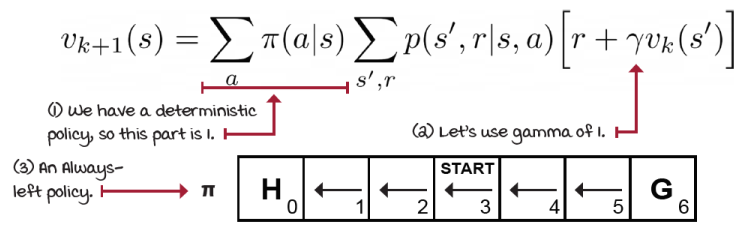
\includegraphics[width=15cm]{images/p000009}
\end{figure}
如上图所示,我们的策略是在每个状态均采取向左的行动,我们假设现在我们在状态5处,根据当前策略,我们只有一个行动既向左行动,同时由于环境具有随机性,使我们可能进入到
状态4(50\%概率)、状态5(33.3\%概率)和状态6(16.6\%概率),初始时,我们设所有状态的状态价值函数的值为0,如下所示:
\begin{equation}
\begin{aligned}
& v_{1}^{\pi}(5) = \sum_{a} \pi (a | s) \sum_{s', r} p(s', r | s, a) \bigg( r + \gamma v_{0}^{\pi}(s') \bigg) \\
& =\sum_{s', r} p(s', r | s, a) \bigg( r + \gamma v_{0}^{\pi}(s') \bigg) & 1  \\
& = p(s'=4, r=0 | s=5, a=Left) (r=0 + 1.0 * v_{0}^{\pi}(4)) & 2 \\
& + p(s'=5, r=0 | s=5, a=Left)(r=0 + 1.0*v_{0}^{\pi}(5)) & 3\\
& + p(s'=6, r=1)(r=1 + 1.0*v_{0}^{\pi}(6)) & 4 \\
& = 0.5*(0 + 0) + 0.33*(0+0) + 0.16*(1+0) = 0.16
\end{aligned}
\label{a-v-f-p-e-swf-demo}
\end{equation}
公式解读如下所示:
\begin{itemize}
    \item 第1行:由于本策略只采取向左行动,因此前面的$\sum_{a}\pi(a | s)$的概率值为1,所以可以去掉;
    \item 第2行:转移到状态4时的情况;
    \item 第3行:转移到状态5时的情况;
    \item 第4行:转移到状态6时的情况;
\end{itemize}
通过上面的计算过程可以看出,我们将初始状态时所有状态的状态价值函数值设置为0,然后通过上面的迭代算法,就可以算出各个状态的状态价值函数的真实值,并且收敛的速度还是
比较快的。
我们首先初始化强化学习环境,我们先安装所需的库:
\lstset{language=BASH, caption={安装依赖库}, label={install-dependency-libs-of-swf}}
\begin{lstlisting}
    cd /e/awork/ext
    git clone https://github.com/mimoralea/gym-walk.git
    cd gym-walk
    pip install .
\end{lstlisting}
环境初始化代码如下所示:
\lstset{language=PYTHON, caption={SWF环境初始化(chp001/exp001\_002.py)}, label={chp001-swf-env-init}}
\begin{lstlisting}
    def startup(self):
        env = gym.make('SlipperyWalkFive-v0')
        P = env.env.P
        init_state = env.reset()
        goal_state = 6
        LEFT, RIGHT = range(2)
        pi = lambda s: {
            0:LEFT, 1:LEFT, 2:LEFT, 3:LEFT, 4:LEFT, 5:LEFT, 6:LEFT
        }[s]
        self.print_policy(pi, P, action_symbols=('<', '>'), n_cols=7)

    def print_policy(self, pi, P, action_symbols=('<', 'v', '>', '^'), 
                n_cols=4, title='Policy:'):
        print(title)
        arrs = {k:v for k,v in enumerate(action_symbols)}
        for s in range(len(P)):
            a = pi(s)
            print("| ", end="")
            if np.all([done for action in P[s].values() 
                        for _, _, _, done in action]):
                print("".rjust(9), end=" ")
            else:
                print(str(s).zfill(2), arrs[a].rjust(6), end=" ")
            if (s + 1) % n_cols == 0: print("|")
\end{lstlisting}
代码解读如下所示:
\begin{itemize}
    \item 第2行:生成强化学习环境,使用的是gmy\_walk包中定义的环境;
    \item 第3行:P为我们在前面讨论的结构:
\lstset{language=PYTHON, caption={SWF环境初始化(chp001/exp001\_002.py)}, label={chp001-swf-env-init}}
\begin{lstlisting}
{
    si:{
        ai: [(p, s', r, False)]
    }
}
\end{lstlisting}

第一层为以状态为键的字典,每个状态是以行动为键的字典,值为一个列表,代表在当前状态下采取行动后,环境会以多大的概
率,转移动新状态,获得的奖励以及新状态是否为终止状态;
\item 第4行:重置环境状态,并获取初始状态;
\item 第5行:将状态6设置为目标状态;
\item 第6行:设置行动LEFT为0,RIGHT为1;
\item 第7$\sim$9行:定义策略,其为lambda表达式,参数为s,定义了一个字典,策略为取出该字典中以参数s为键的元素,其中s代表状态编号,策略的类型为函数;
\item 第10行:打印策略;
\item 第12、13行:定义打印策略函数:,
\begin{itemize}
    \item pi为策略类型为函数,参数为状态编号,返回值为所采取的行动;
    \item P为状态、行动的转移矩阵,即环境的MDP特性;
    \item action\_symbols 行动的符号表示;
    \item n\_cols 共有几个状态,这里有7个状态,0和6代表终止状态;
    \item title 标题;
\end{itemize}
\item 第15行:arrs的形式为:{0: '<', 1: '>'};
\item 第16行:循环处理每个状态,s为状态编号;
\item 第27行:以状态编号为参数,调用策略函数,求出该状态下采取的行动编号(在其他复杂问题中,可能是采取一系列行动的概率分布);
\item 第19、20行:
通过如下代表:
\lstset{language=PYTHON, caption={SWF环境初始化(chp001/exp001\_002.py)}, label={chp001-swf-env-init-test001}}
\begin{lstlisting}
def test001(self, P, state):
    v1 = [action for action in P[state].values()]
    print('v1: {0};'.format(v1))
    v2 = [done for action in P[state].values() for _, _, _, done in action]
    print('v2: {0};'.format(v2))
    v3 = np.all(v2)
    print('v3: {0};'.format(v3))
\end{lstlisting}    
状态0时:
\lstset{language=PYTHON, caption={SWF环境初始化(chp001/exp001\_002.py)}, label={chp001-swf-env-init-test001-1}}
\begin{lstlisting}
    v1: [
            [
                (0.5000000000000001, 0, 0.0, True), 
                (0.3333333333333333, 0, 0.0, True), 
                (0.16666666666666666, 0, 0.0, True)
            ], 
            [
                (0.5000000000000001, 0, 0.0, True), 
                (0.3333333333333333, 0, 0.0, True), 
                (0.16666666666666666, 0, 0.0, True)
            ]
        ];
    v2: [True, True, True, True, True, True];
    v3: True;
\end{lstlisting}
状态1时:
\lstset{language=PYTHON, caption={SWF环境初始化(chp001/exp001\_002.py)}, label={chp001-swf-env-init-test001-2}}
\begin{lstlisting}
    v1: [
            [
                (0.5000000000000001, 0, 0.0, True), 
                (0.3333333333333333, 1, 0.0, False), 
                (0.16666666666666666, 2, 0.0, False)
            ], 
            [
                (0.5000000000000001, 2, 0.0, False), 
                (0.3333333333333333, 1, 0.0, False), 
                (0.16666666666666666, 0, 0.0, True)
            ]
        ];
    v2: [True, False, False, False, False, True];
    v3: False;
\end{lstlisting}
状态2时:
\lstset{language=PYTHON, caption={SWF环境初始化(chp001/exp001\_002.py)}, label={chp001-swf-env-init-test001-3}}
\begin{lstlisting}
    v1: [
            [
                (0.5000000000000001, 1, 0.0, False), 
                (0.3333333333333333, 2, 0.0, False), 
                (0.16666666666666666, 3, 0.0, False)
            ], 
            [
                (0.5000000000000001, 3, 0.0, False), 
                (0.3333333333333333, 2, 0.0, False), 
                (0.16666666666666666, 1, 0.0, False)
            ]
        ];
    v2: [False, False, False, False, False, False];
    v3: False;
\end{lstlisting}
上面的代码就是确定某个状态是否是终止状态;
\item 第21行:当为终止状态时打印空;
\item 第23行:当不为终止状态时,打印状态编号和行动的符号;
\end{itemize}
下面我们来看我们取得胜利的概率,如下所示:
\lstset{language=PYTHON, caption={求获得胜利既到达状态6的概率(chp001/exp001\_002.py)}, label={chp001-swf-win-prob}}
\begin{lstlisting}
    def probability_success(self, env, pi, goal_state, n_episodes=100, max_steps=200):
        random.seed(123); np.random.seed(123) ; env.seed(123)
        results = []
        for epoch in range(n_episodes):
            state, done, steps = env.reset(), False, 0
            while not done and steps < max_steps:
                state, _, done, h = env.step(pi(state))
                steps += 1
            results.append(state == goal_state)
        return np.sum(results)/len(results)
\end{lstlisting}
代码解读如下所示:
\begin{itemize}
    \item 第4行:循环指定epoch数;
    \item 第5行:初始化环境,我们假定开始时Agent在状态3;
    \item 第6行:完整执行一个epoch,并且如果超过指定步数后,强制终止此epoch;
    \item 第7行:在当前状态state下,根据策略pi,采取一个行协pi(state),调用环境的evn.step方法,转移到下一个状态,其返回值为:下一状态、奖励、是否完结、附加信息,其中新状态和奖励是根据我们状态转移P来决定的;
    \item 第8行:统计当前epoch中的步数;
    \item 第9行:当完成一个epoch后,如果终止状态为Goal状态,则将1加入到results列表中,否则将0加入到results列表中;
    \item 第10行:results列表中为1的项数除以总项数即为获胜的概率;
\end{itemize}
接下来我们看一下在该策略下,我们可以获取平均回报:
\lstset{language=PYTHON, caption={求平均回报(chp001/exp001\_002.py)}, label={chp001-swf-mean-return}}
\begin{lstlisting}
    def mean_return(self, env, pi, n_episodes=100, max_steps=200):
        random.seed(123); np.random.seed(123) ; env.seed(123)
        results = []
        for _ in range(n_episodes):
            state, done, steps = env.reset(), False, 0
            results.append(0.0)
            while not done and steps < max_steps:
                state, reward, done, _ = env.step(pi(state))
                results[-1] += reward
                steps += 1
        return np.mean(results)
\end{lstlisting}
这段代码的逻辑与\ref{chp001-swf-win-prob}类似,只不过是每个epoch开始前,向results列表中加入一个0.0元素,在该epock中的每一步,都会将所获得奖励reward叠加到该值上,这样可以求出每个epoch的
累积奖励,最后我们返回这些累积奖励值的平均值。
接下来我们对当前策略进行评估,利用迭代法求出所状态价值函数的值:
\lstset{language=PYTHON, caption={策略评估(chp001/exp001\_002.py)}, label={chp001-policy-evaluation}}
\begin{lstlisting}
    def policy_evaluation(self, pi, P, gamma=1.0, theta=1e-10):
        prev_V = np.zeros(len(P), dtype=np.float64)
        while True:
            V = np.zeros(len(P), dtype=np.float64)
            for s in range(len(P)):
                for prob, next_state, reward, done in P[s][pi(s)]:
                    V[s] += prob * (reward + gamma * prev_V[next_state] * (not done))
            if np.max(np.abs(prev_V - V)) < theta:
                break
            prev_V = V.copy()
        return V
\end{lstlisting}
代码解读如下所示:
\begin{itemize}
    \item 第2行:初始时将所有状态的状态价值函数的值设置为0,将其作为上一迭代的值;
    \item 第4行:进行无限次迭代循环;
    \item 第5行:当前状态的状态价值函烽的初始值置为0;
    \item 第6行:对每个状态进行循环;
    \item 第7行:对每个状态,在当前策略下采取的行动,根据转移函数P,得到概率prob,下一个状态next\_state和奖励reward,以及是否结束标志done;
    \item 第8行:利用公式$v_{k+1}=\sum_{a} \pi(a|s) \sum_{s',r} (r + \gamma v_{k})$求出新的状态价值函数的值;
    \item 第8、9行:当求完所有状态的状态价值函数值时,看两次迭代之间状态价值函数的差值是否小于阈值,如果小于则退出最外层的无限循环;
    \item 第10行:如果二者的差值大于阈值,则将当前值设置为上一次迭代值,重复进行循环;
\end{itemize}
上面程序的最终结果就是求出所有状态的真实的状态价值函数的值,接下来我们打印状态价值函数的值:
\lstset{language=PYTHON, caption={打印状态价值函数的值(chp001/exp001\_002.py)}, label={chp001-print-state-value-function}}
\begin{lstlisting}
    def print_state_value_function(self, V, P, n_cols=4, prec=3, title='State-value function:'):
        print(title)
        for s in range(len(P)):
            v = V[s]
            print("| ", end="")
            if np.all([done for action in P[s].values() for _, _, _, done in action]):
                print("".rjust(9), end=" ")
            else:
                print(str(s).zfill(2), '{}'.format(np.round(v, prec)).rjust(6), end=" ")
            if (s + 1) % n_cols == 0: print("|")

    def startup(self):
        env = gym.make('SlipperyWalkFive-v0')
        P = env.env.P
        init_state = env.reset()
        goal_state = 6
        LEFT, RIGHT = range(2)
        pi = lambda s: {
            0:LEFT, 1:LEFT, 2:LEFT, 3:LEFT, 4:LEFT, 5:LEFT, 6:LEFT
        }[s]
        self.print_policy(pi, P, action_symbols=('<', '>'), n_cols=7)
        prob = self.probability_success(env, pi, goal_state)
        print('win prob:{0};'.format(prob))
        g_mean = self.mean_return(env, pi)
        print('mean return:{0};'.format(g_mean))
        V = self.policy_evaluation(pi, P)
        self.print_state_value_function(V, P, n_cols=7, prec=5)
        improved_pi = self.policy_improvement(V, P)
        self.print_policy(improved_pi, P, action_symbols=('<', '>'), n_cols=7)
\end{lstlisting}
这个函数比较简单,我们就不做介绍了。
通过对策略的评价,我们得到了每个状态的状态价值函数的值,接下来我们讨论怎样根据这些内容来优化我们的策略。这里我们需要用到行动函数,即在每个状态,我们从所有行动中,找出可以使我们转到的新状态,
可以获得最高的状态价值函数,并以此为新的策略:
\begin{equation}
\begin{aligned}
& \pi ' (s) = \arg \max_{a} \sum_{s',r} p(s', r | s, a)(r + \gamma v_{\pi}(s'))
\end{aligned}
\label{a-v-f-p-e-swf-demo}
\end{equation}
上式中的$\pi '(s)$就是改进后的策略。策略改进代码如下所示:
\lstset{language=PYTHON, caption={策略改进(chp001/exp001\_002.py)}, label={chp001-policy-improvement}}
\begin{lstlisting}
    def policy_improvement(V, P, gamma=1.0):
        Q = np.zeros((len(P), len(P[0])), dtype=np.float64)
        for s in range(len(P)):
            for a in range(len(P[s])):
                for prob, next_state, reward, done in P[s][a]:
                    Q[s][a] += prob * (reward + 
                            gamma * V[next_state] * (not done))
        new_pi = lambda s: {s:a for s, a 
            in enumerate(np.argmax(Q, axis=1))
        }[s]
        return new_pi
\end{lstlisting}
代码解读如下所示:
\begin{itemize}
    \item 第2行:Q为一个二维数组,第一维是所有的状态,第二维是在某个状态下所有的行动选项,其值为该行动的行动价值函数,初始时设置为0;
    \item 第3行:循环处理所有状态:
    \item 第4行:循环处理每个状态下可以采取的所有行动:
    \item 第5行:根据环境的状态转移函数,在该状态下采取该行动,可以得到:转移到新状态的概率、新状态、奖励、是否为终止状态;
    \item 第6、7行行:根据公式$q_{\pi}(s, a)=\sum_{s',r} p(s', r|s, a)(r+\gamma v_{\pi}(s'))$;
    \item 第8$\sim$10行:求出新的优化过的策略:
\begin{equation}
\begin{aligned}
    \begin{bmatrix}
        q(s_{0}, a_{0}) & q(s_{0}, a_{1}) & ... & q(s_{0}, a_{k_{0}}) \\
        q(s_{1}, a_{0}) & q(s_{1}, a_{1}) & ... & q(s_{1}, a_{k_{1}}) \\
        ... & ... & ... & ... \\
        q(s_{l}, a_{0}) & q(s_{l}, a_{1}) & ... & q(s_{l}, a_{k_{l}}) \\
    \end{bmatrix}
\end{aligned}
\label{chp001-policy-improvement1}
\end{equation}
上式中每一行代表一个状态,每一列代表在该状态下采取某个行动可以获取到的累积回报,注意每行的数量可能并不相同。np.argmax(,axis=1)代表把第2维去掉,即求每一行
的最大值,也就是求出某个状态采取什么行动可以获得最大的回报。最终形厉每个状态应该采取的行动编号,利用lambda表达式形成策略函数。
    ;
    \item 第11行:返回这个新生成的策略函数;
\end{itemize}
运行结果如下所示:
\begin{figure}[H]
	\caption{Slippery Walk Floor策略优化一次结果}
	\label{p000010}
	\centering
	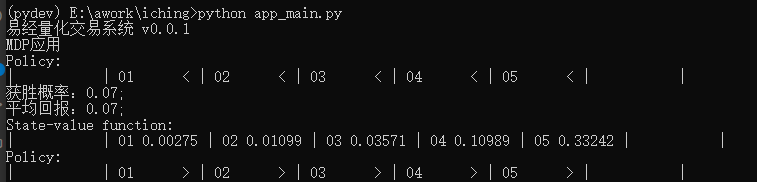
\includegraphics[width=15cm]{images/p000010}
\end{figure}
如上图可以看出,仅经过一次策略优化,我们就可以得到正确的策略。
实际上我们对策略优化之后,我们可以重新进行策略评估,然后再进行优化,形成所谓的策略迭代,程序如下所示:
\lstset{language=PYTHON, caption={策略迭代(chp001/exp001\_002.py)}, label={chp001-policy-iteration}}
\begin{lstlisting}
    def policy_iteration(self, P, gamma=1.0, theta=1e-10):
        random_actions = np.random.choice(tuple(P[0].keys()), len(P))
        pi = lambda s: {s:a for s, a in enumerate(random_actions)}[s]
        while True:
            old_pi = {s:pi(s) for s in range(len(P))}
            V = self.policy_evaluation(pi, P, gamma, theta)
            pi = self.policy_improvement(V, P, gamma)
            if old_pi == {s:pi(s) for s in range(len(P))}:
                break
        return V, pi

    def startup(self):
        env = gym.make('SlipperyWalkFive-v0')
        P = env.env.P
        init_state = env.reset()
        goal_state = 6
        LEFT, RIGHT = range(2)
        pi = lambda s: {
            0:LEFT, 1:LEFT, 2:LEFT, 3:LEFT, 4:LEFT, 5:LEFT, 6:LEFT
        }[s]
        self.print_policy(pi, P, action_symbols=('<', '>'), n_cols=7)
        prob = self.probability_success(env, pi, goal_state)
        print('win prob:{0};'.format(prob))
        g_mean = self.mean_return(env, pi)
        print('mean return:{0};'.format(g_mean))
        V = self.policy_evaluation(pi, P)
        self.print_state_value_function(V, P, n_cols=7, prec=5)
        improved_pi = self.policy_improvement(V, P)
        self.print_policy(improved_pi, P, action_symbols=('<', '>'), n_cols=7)
        # policy iteration
        optimal_V, optimal_pi = self.policy_iteration(P)
        self.print_policy(optimal_pi, P, action_symbols=('<', '>'), n_cols=7)
        self.print_state_value_function(optimal_V, P, n_cols=7, prec=5)
\end{lstlisting}
代码解读如下所示:
\begin{itemize}
    \item 第2行:其中P[0]={0:[(0.5, 0, 0.0, True), ...], 1:[...]},所以tuple(P[0].keys())为(0, 1),因此np.random.choice为生成长度为len(P)既所有状态数的数组,数组的每一位由(0,1)中随机抽取;
    \item 第3行:生成策略的lambda表达式,参数为状态编号;
    \item 第4行:进入无限循环:
    \item 第5行:将当前策略保存为原始策略,类型为字典,格式为:{状态: 行动};
    \item 第6行:求出在当前策略下的状态价值函数;
    \item 第7行:根据状态价值函数得到优化后的策略;
    \item 第8、9行:将优化后策略也转为格式为{状态: 行动}的字典,与原来的策略形成的字典进行比较,如果相等则意味着找到了最佳策略,则退出无限循环,否则继续循环优化;
\end{itemize}
运行结果如下所示:
\begin{figure}[H]
	\caption{Slippery Walk Floor策略迭代结果}
	\label{p000011}
	\centering
	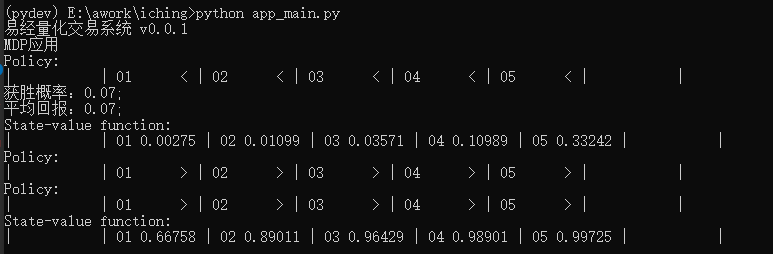
\includegraphics[width=15cm]{images/p000011}
\end{figure}
上面讲的是策略迭代算法(PI:Policy Iteration),其核心思想是先根据策略求出状态价值函数,然后根据状态价值函数,在每个状态下选择能够达到最大状态价值函数状态的行动,形成优化后的策略,
然后循环执行上述过程。但是这种方法通常收敛速度较慢,我们接下来介绍值迭代算法(VI:Value Iteration)。
\subsection{值迭代(VI)}
值迭代(VI: Value Iteration)的核心思想是先令所有状态的状态价值函数值为0.0,在每个状态下求出所采取的行动的回报,找到得到最大回报的行动,根据下面的公式确定新的状态价值函数值:
\begin{equation}
\begin{aligned}
    v_{k+1}=\max_{a} \sum_{s',r} p(s', r | s, a)\bigg( r + \gamma v_{k}(s') \bigg)
\end{aligned}
\label{chp001-value-iteration-formula}
\end{equation}
代码实现如下所示:
\lstset{language=PYTHON, caption={策略迭代(chp001/exp001\_002.py)}, label={chp001-value-iteration}}
\begin{lstlisting}
    def value_iteration(self, P, gamma=1.0, theta=1e-10):
        V = np.zeros(len(P), dtype=np.float64)
        while True:
            Q = np.zeros((len(P), len(P[0])), dtype=np.float64)
            for s in range(len(P)):
                for a in range(len(P[s])):
                    for prob, next_state, reward, done in P[s][a]:
                        Q[s][a] += prob * (reward + gamma * V[next_state] * (not done))
            if np.max(np.abs(V - np.max(Q, axis=1))) < theta:
                break
            V = np.max(Q, axis=1)
        pi = lambda s: {s:a for s, a in enumerate(np.argmax(Q, axis=1))}[s]
        return V, pi

    def startup(self):
        env = gym.make('SlipperyWalkFive-v0')
        P = env.env.P
        init_state = env.reset()
        goal_state = 6
        LEFT, RIGHT = range(2)
        pi = lambda s: {
            0:LEFT, 1:LEFT, 2:LEFT, 3:LEFT, 4:LEFT, 5:LEFT, 6:LEFT
        }[s]
        self.print_policy(pi, P, action_symbols=('<', '>'), n_cols=7)
        prob = self.probability_success(env, pi, goal_state)
        print('win prob: {0};'.format(prob))
        g_mean = self.mean_return(env, pi)
        print('mean return: {0};'.format(g_mean))
        V = self.policy_evaluation(pi, P)
        self.print_state_value_function(V, P, n_cols=7, prec=5)
        improved_pi = self.policy_improvement(V, P)
        self.print_policy(improved_pi, P, action_symbols=('<', '>'), n_cols=7)
        # policy iteration
        print('PI: Policy Iteration')
        optimal_V, optimal_pi = self.policy_iteration(P)
        self.print_policy(optimal_pi, P, action_symbols=('<', '>'), n_cols=7)
        self.print_state_value_function(optimal_V, P, n_cols=7, prec=5)
        print('VI: Value Iteration')
        V2, pi2 = self.value_iteration(P)
        self.print_policy(optimal_pi, P, action_symbols=('<', '>'), n_cols=7)
        self.print_state_value_function(optimal_V, P, n_cols=7, prec=5)
\end{lstlisting}
代码解读如下所示:
\begin{itemize}
    \item 第2行:初始状态下状态价值函数值为0.0;
    \item 第3行:无限循环求解状态价值函数和策略:
    \item 第4行:初始化$q(s,a)$函数,第0维是状态,第1维是行动,初始值为0.0;
    \item 第5、6行:循环处理每个$(s, a)$组合:
    \item 第7行:当在状态$s$采取行动$a$后,环境会转移到新状态$s'$并给出奖励$r$,用环境P中的$(prob, s', r, isTerminal)$来表示,
    其中prob为转移到新状态$s'$并获取奖励$r$的概率,最后一项表示$s'$是否是终止状态;
    \item 第8行:利用公式$q(s, a) = \sum_{s',r} p(s',r|s,a)(r+\gamma v_{\pi}(s'))$,求出Q函数的值;
    \item 第9、10行:如果上一步得到状态价值函数值,与Q函数值对每个状态采取行动可以获得最大Q函数值所组成的新状态价值函数值之间
    的差距小于阈值时终止最外层无限循环;
    \item 第11行:对于每个状态,用采取所有行动中取得最大Q值作为状态价值函数的值;
    \item 第12行:当结束无限循环之后,将策略定为在每个状态,取可以取得最大Q值的行动作为应该选取的行动;
\end{itemize}